\documentclass[11pt,letterpaper]{article}

%%%%%%%%%%%%%%%%%%%%%%%%%%%%%%%%%%%%%%%%%%%%%%%%%%%%%%%%%%%%%%%%%%%%%%%%%
\pagestyle{plain}                                                      %%
%%%%%%%%%% EXACT 1in MARGINS %%%%%%%                                   %%
\setlength{\textwidth}{6.5in}     %%                                   %%
\setlength{\oddsidemargin}{0in}   %% (It is recommended that you       %%
\setlength{\evensidemargin}{0in}  %%  not change these parameters,     %%
\setlength{\textheight}{8.5in}    %%  at the risk of having your       %%
\setlength{\topmargin}{0in}       %%  proposal dismissed on the basis  %%
\setlength{\headheight}{0in}      %%  of incorrect formatting!!!)      %%
\setlength{\headsep}{0in}         %%                                   %%
\setlength{\footskip}{.5in}       %%                                   %%
%%%%%%%%%%%%%%%%%%%%%%%%%%%%%%%%%%%%                                   %%
%\newcommand{\required}[1]{\section*{\hfil #1\hfil}}                    %%
\renewcommand{\refname}{\hfil References Cited\hfil}                   %%
%\bibliographystyle{plain}                                              %%
%%%%%%%%%%%%%%%%%%%%%%%%%%%%%%%%%%%%%%%%%%%%%%%%%%%%%%%%%%%%%%%%%%%%%%%%%

%PUT YOUR MACROS HERE

\usepackage{amsmath}
\usepackage{amsfonts}
\usepackage{amssymb}
\usepackage{graphicx}
\usepackage{ulem}
\usepackage[hidelinks]{hyperref}


\title{Magnetometry}


\author{Ian Hunt-Isaak\\ \begin{small}
Partner: Corina Miner
\end{small}}

\begin{document}


\date{}
\maketitle
\section{} %1



\section{} %2


\section{} %3

\section{} %4

\section{}%5
A Hall Effect Gaussmeter works on the principle of the Lorentz force of a magnetic field acting on a moving charge. Placing a metallic strip of significant width in a magnetic field and running current through it will cause the Lorentz force to act on the charge carriers in the metal. The component of the field normal to the surface of the strip will cause a charge imbalance to develop accross the width of the strip, this can be visualized in Fig. \ref{fig:hall_effect}. By measuring the voltage generated by the charge imbalance, $V_H$ in Fig. \ref{fig:hall_effect}, and knowing the magnitude of the current and properties such as the charge carrier density of the material we can determine the magnitude of the magnetic field normal to the strip. The fact that a hall effect can only measure the field normal to strip is why it matters how the probe is inserted in the field. If the probe is tilted relative to the field the measurment of the field will be reduced from the actual field value.
\begin{figure}[h!]
  \centering
      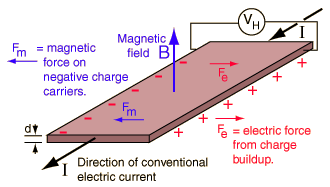
\includegraphics[scale=.8]{hall.png}
      \caption{Image from {\url http://hyperphysics.phy-astr.gsu.edu/hbase/magnetic/imgmag/hall.gif}}
      \label{fig:hall_effect}
\end{figure}

\end{document}